\chapter{Coverage Path Planning}
\label{cha:cpp}

The main focus of this thesis is coverage path planning of outdoor multi-floor environments. This chapter describes implementation details of existing CPP algorithms and theory for new algorithms proposed in this project.

\section{Environment representation}
The main problem with CPP over multiple floors is the representation of the environment. 

One approach is to make a 2D plane representation of each floor, but this requires floor segmentation. The problem with floor segmentation is that it is not always trivial where to split the floors. An example is a spiral ramp in a parking garage. Another disadvantage is that it would make a plan for each floor separately and not take the full path over multiple floors into consideration when optimising the path. 

Another approach could be to transform the point cloud into a voxel grid with algorithms such as OctoMap \cite{octomap}. This method however, transforms multiple points into boxes, which means that information gets lost. 

Taking these arguments into consideration, the representation of the environment in this project was chosen to be a point cloud with classified points. The points were classified as $Coverable$, $Traversable$ and $Inaccessible/Obstacle$, see details and definitions in Chapter \ref{cha:terain_assessment}. No discretizations were made and all calculations were directly made on the points in the point cloud.

\section{Motion Planner}
 \label{sec:motion_planner}
The motion planning is an important base of many coverage path planning algorithms. It solves the problem of planning the shortest obstacle free path between two given points. The same motion planner was used for all implemented algorithms. It was based on A* described in algorithm \ref{alg:astar} to find the shortest path and A*SPT, see algorithm \ref{alg:astarSPT} to make the path smoother. If no path was found by the A*, the RRT algorithm, see Algorithm \ref{alg:RRT} was used. It is more reliable but does not generate the optimal path. 

To find neighbour positions of a point is a function that is frequently used in both motion planning and in CPP. The neighbours of a position were given by taking a step in 8 directions from the position and taking the closest $Traversable$ point from that spot, see Figure \ref{fig:extend}

\begin{figure}
    \centering
    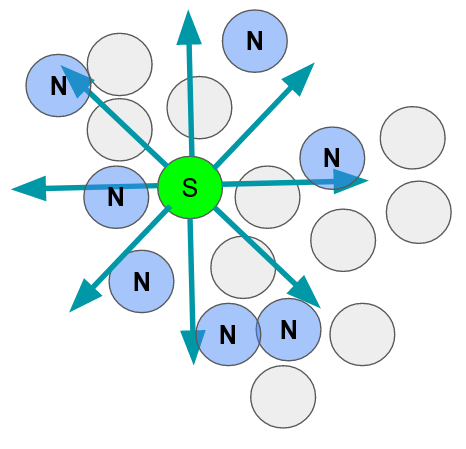
\includegraphics[width=\0.5\textwidth]{figures/neighbours.png}
    \caption{Neighbour positions, $N$, of a point $S$, were generated by taking a step in 8 directions from $S$ and choosing the closest $Traversable$ point. All points in the figure are $Traversable$.}
    \label{fig:my_label}
\end{figure}

Another task that is common and handled by the Motion Planner is to check the validity of a path between two points. This function assumes that the two points are $Traversable$. The validation is described in detail in algorithm \ref{alg:is_valid_step}. If the closest traversable point is the same as the original point it means that this point is on the border between traversable and untraversable space, and that the path should not be valid. However, if the distance is smaller than the resolution, the step size, the path is traversable. If the distance between two points is bigger, the line-of-sight path between these points is divided into small steps and is only valid if every step ends on a position close to a traversable point, see figure \ref{fig:isvalidstep}. 

\begin{figure}
    \centering
    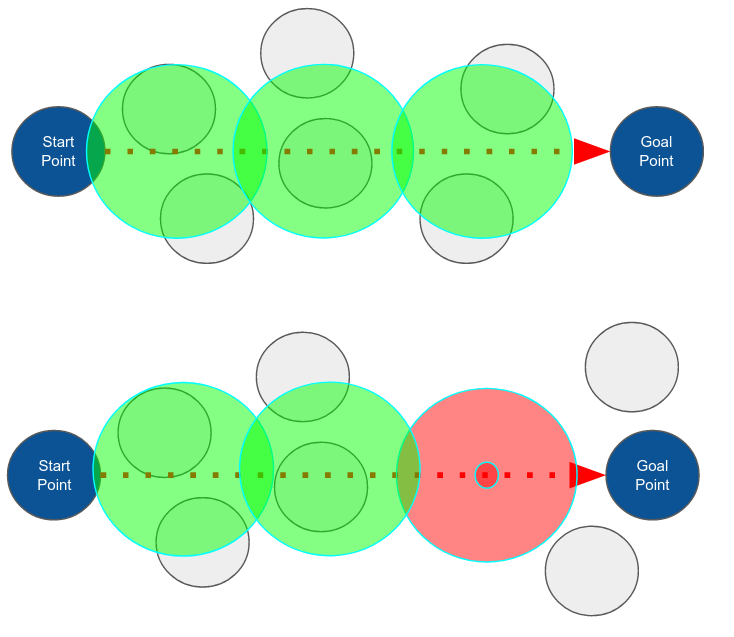
\includegraphics[width=0.7\textwidth]{figures/isvalidstep.png}
    \caption{An example of a valid (upper illustration) and an invalid (lower illustration) step between two points. The line-of-sight path between the points are divided into three steps. At each step the algorithm calculates the distance to the closest traversable point. If the distance is bigger than the untraversability threshold (see red circle in lower illustration) the path will be classified as invalid.}
    \label{fig:isvalidstep}
\end{figure}

\begin{algorithm}[H]
\SetAlgoLined
\KwData{Start point, $p_{s}$, Goal point, $p_g$, Step size $\lambda$, Threshold radius for untraversability, $r_{trav}$}
\KwResult{A boolean, representing whether the path is valid or not.}
\If{\textup{$p_{g}$ is $p_{s}$ }}{
    \textup{\textbf{return }$False$} \\
}
$d_{tot} = \abs{p_{g} - p_{s}}$ \\
\If{\textup{$d_{tot} < \lambda$ }}{
    \textup{\textbf{return} $True$} \\
}
$N_{steps} = d_{tot} / \lambda$ \\
$\vec{D}$ = \textup{Direction vector from $p_s$ to $p_g$ of length $\lambda$ } \\
\For{\textup{step $i \in 1, 2, ..., N_{steps}$}}{

    \textup{Set $s_i$ \rightarrow  $p_{s}$ + $i \cdot \vec{D}$ } \\
    \If{\textup{Distance to nearest traversable point to $s_i$ > $r_{trav}$}}{
        \textup{\textbf{return }$False$} \\
    } 
}
\textup{\textbf{return} $True$}
 \caption{Algorithm that returns if a step between two points is valid or not.}
 \label{alg:is_valid_step}
\end{algorithm}

\section{RRT implementation (Will probably be removed)}
One of the simplest solutions to the coverage path planning problem is to make a RRT tree that covers the area and then visit every point. Algorithm \ref{alg:build_tree} was used to build up the tree. It simply picks a random traversable point and uses $Extend$, see algorithm \ref{alg:extend} to expand the tree towards the random point. This is done until the desired coverage or a maximum amount of iterations has been reached.

\begin{algorithm}[H]
\SetAlgoLined
\KwData{Start point, $p_{s}$}
\KwResult{Search tree, $T$}
T \leftarrow p_s \\
\While{\textup{Coverage or maximum iterations reached}}{
    p_{rand} = \textup{Random traversable point in point cloud}\\
    p_{new} = Extend(T, p_{rand})\\
    \If{\textup{$p_{new}$ is $Trapped$}}{
        \textup{\textbf{continue}} \\
    }
    T \leftarrow p_{new}
}
\textup{\textbf{return $T$}}
 \caption{Algorithm that builds up a search tree with RRT}
 \label{alg:build_tree}
\end{algorithm}

The next step is to find a path that visits every node in the tree. This could be done by a simple Deep First Algorithm, see \ref{alg:find_path_through_tree}. At first all points are visited in a deep first order. When all points have been visited a path is generated. To make sure the path is obstacle free, A* of the Motion Planner is used to generate a feasible path between the points.

\begin{algorithm}[H]
\SetAlgoLined
\KwData{Search tree, $T$, starting point $p_s$}
\KwResult{Path through tree, $P$}
Q \leftarrow $p_s$ \\
V \leftarrow $p_s$ \\
\While{\textup{$Q$ is not empty}}{
    $p$ = $Pop(Q)$ \\
    V \leftarrow $p$ \\
    \For{\textup{neighbour $n$ of $p$}}{
        \If{\textup{$n$ is not in $V$}}{
            Q \leftarrow $n$ \\
        }
    }
}
\For{\textup{point $p \in V$}}{
    \textup{$P \leftarrow$ Path from last point in $P$ to $p$ using A*} \\
}
\textup{\textbf{return $P$}}
 \caption{Deep First Algorithm. Generates a path through a search tree}
 \label{alg:find_path_through_tree}
\end{algorithm}

\section{Coverage Path Planner}
\label{sec:general_cpp}
The main focus of this project was to evaluate different CPP algorithms. These algorithms had many common functions that are used to calculate the path that covers the area. The algorithms BA* and Inward Spiral that were described in section \ref{sec:BAstar} and \ref{sec:spiral} are based on a two dimensional world representation with tiles. To make them applicable directly on a point cloud and efficient in a multi floor environment following general modifications were to be made.

\begin{itemize}
    \item Instead of moving between tiles $c$, the path $P$ consisted of $Traversable$ points $p$.
    \item To keep track of covered areas, BA* adds tiles to a model and Spiral marks cells as visited. Instead, this was handled by marking all coverable points within a radius, $r_R$ from the visited position as \emph{covered}. When covering a path between two points, positions along the path were visited as well with such frequency that it made sure that all points along the path within the radius were covered.
    \item A point was classified as \emph{visited} if the distance to the closest point in the visited path $P$ was smaller than a threshold $r_{visited}$.
    \item Getting neighbour positions is a used function in both A* and Inward Spiral. Instead of receiving tiles nearby in each of the forth directions this function returned $Traversable$ points in 8 directions, as previously described in Section \ref{sec:motion_planner}.
    \item A neighbour point was \emph{blocked} if the point was classified as \emph{visited} or if the path to the point was classified as \emph{invalid} by Algorithm \ref{alg:is_valid_step}.
\end{itemize}

The two algorithms BA* and Inward Spiral has the same structure, but different ways of solving following steps:
\begin{enumerate}
    \item \textbf{CPP Step 1} - Find a path that covers the area until it reaches a dead end. Follow the path.
    \item \textbf{CPP Step 2} - Find a new starting point.
    \item \textbf{CPP Step 3} - Find the shortest path from the dead end to the next starting point. Follow the path and go back to CPP Step 1.
\end{enumerate}

\section{BA* implementation}
\label{sec:BA*impl}
This section describes details about the implementation of BA* algorithm. The implementation of CPP Step 1 was mostly based on Algorithm \ref{alg:BM}. Since the number of neighbours was eight instead of four the priority order was set to north, south, northeast, northwest, southeast, southwest, east, west. The used BM algorithm is described in Algorithm \ref{alg:newBM}. CPP Step 2 and 3 were implemented according to section \ref{sec:BAstar}, with the modifications described in section \ref{sec:general_cpp}. An illustration that shows a simplified plan of the implemented BA* is shown in Figure \ref{fig:examplebastar}.

\begin{algorithm}[H]
\SetAlgoLined
\KwData{Starting point, $p_{sp}$. Traversable point cloud $P_{trav}$}
\KwResult{Covering path $P_{local}$}
\textup{Set $CriticalPointFound \rightarrow false$} \\
$p_{curr}$ = $p_{sp}$ \\
$P_{local} = \emptyset $\\
\While{\textup{$CriticalPointFound$ is $false$}}{
    \textup{Set $CriticalPointFound \rightarrow true$} \\
    \For{\textup{point} $p_n \in P_{trav}$ \textup{in direction $n \in$ north, south, northeast, northwest, southeast, southwest, east, west from $p_{curr}$}}{
        \If{\textup{$p_n$ is not \emph{blocked}}}{
            $P_{local}.\texttt{push\_back}(p_n)$ \\
            $p_{curr}$ = $p_{n}$ \\
            \textup{Set $CriticalPointFound \rightarrow false$} \\
            \textbf{\textup{break}} \\
        }
    }
}
\textup{\textbf{return}} $P_{local}$

 \caption{CPP Step 1 for BA*. A modified BM algorithm (Algorithm \ref{alg:BM})}
 \label{alg:newBM}
\end{algorithm}


\begin{figure}
    \centering
    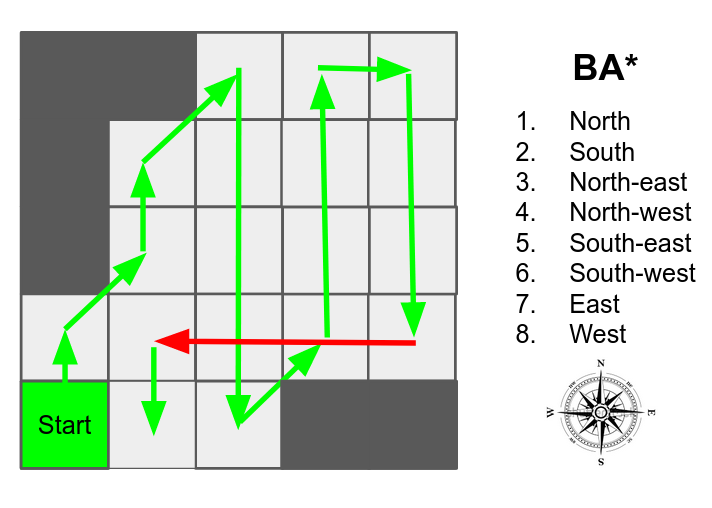
\includegraphics[width=0.6\textwidth]{figures/examplebastar.png}
    \caption{An illustration how the BA* algorithm would solve the CPP. Green arrows are the main path that covers new points. When reaching a dead zone, the robot needs to travel to a new uncovered spot. Red arrows are symbolising these movements when no new points are covered.}
    \label{fig:examplebastar}
\end{figure}



\section{Spiral implementation}
\label{sec:spiral_impl}
 The implementation of the Inward spiral algorithm was based on Section \ref{sec:spiral}. Just like in the BA* implementation the number of neighbours were increased and the priority order had to be changed. The priority for the neighbours were set to backwards-right, right, forward-right, forward, forward-left, left, backwards-left. CPP Step 1  was implemented by applying this change of priority and the modifications in Section \ref{sec:general_cpp} to Algorithm \ref{alg:inwardspiral}. Wavefront algorithm, Algorithm \ref{alg:wavefront}, was implemented with the same modifications for the CPP Step 2. For CPP Step 3, the same solution was implemented as for the BA*. Unlike the original description of the Inward Spiral algorithm in Section \ref{sec:spiral}, the smoothing of the path, see Algorithm \ref{alg:astarSPT}, was applied on the A* path in the implementation.  An illustration that shows a simplified plan of the implemented Inward Spiral is shown in Figure \ref{fig:examplespiral}.

\begin{figure}
    \centering
    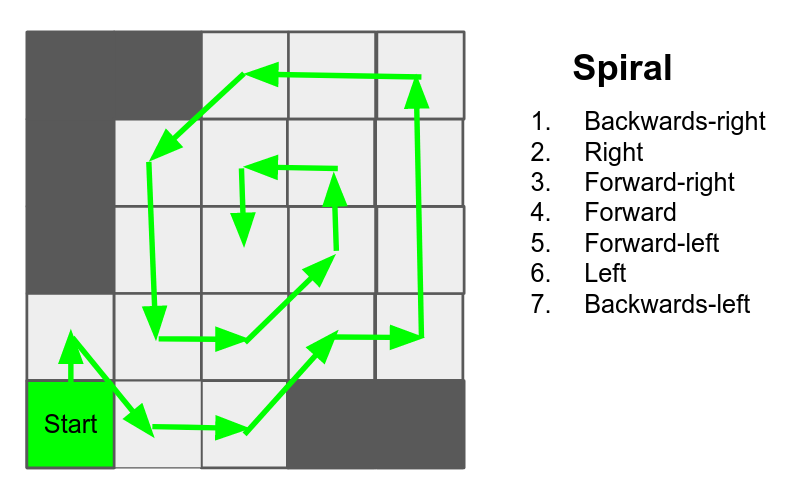
\includegraphics[width=0.6\textwidth]{figures/examplespiral.png}
    \caption{An illustration how the Spiral algorithm would solve the CPP. Green arrows are the main path that covers new points.}
    \label{fig:examplespiral}
\end{figure}

\section{Curved BA*}
The BA* algorithm generates straight zig-zag paths across the area, while the Inward Spiral follows the walls of the environment and goes in a spiral motion towards the center. The advantage of BA* path is the straight paths that are optimal for cleaning and works good on big open areas. However, a real world outdoor environment has many obstacles and uneven walls that requires the path to adjust to the environment. This is better done by the Inward Spiral. 

Curved BA* is a variation of BA*, which according to the author's knowledge has not been tested before. The idea of Curved BA* is to cover environments such as multi floor parking garages that consists of both open areas and many obstacles. 

When the normal BA* is applied to an environment with obstacles, small uncovered missed spots appears between the paths, see Figure \ref{fig:bastarfail}. This spots needs to be visited separately, which makes the path longer and the algorithm less effective. A possible solution to this problem is to adjust the priority order to fill the missed spots right away. In Curved BA* priority order of the neighbours were changed to west, northwest, southwest, north, south, northeast, southeast, east. Except this change, CPP Step 1-3 are identical to the BA* implementation (Section \ref{sec:BA*impl}). This algorithm generated a zig-zag path that was more fitted to the environment, see example in figure \ref{fig:examplebastarvariant}.

\begin{figure}
    \centering
    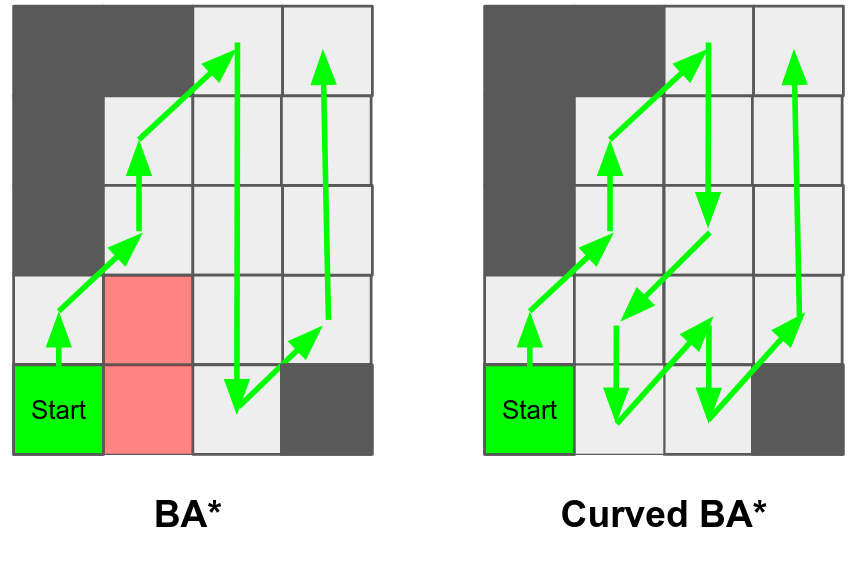
\includegraphics[width=0.6\textwidth]{figures/bastarfail.png}
    \caption{Difference between BA* and Curved BA*. BA* misses spots (red area) that has to be covered later, which is less effective.}
    \label{fig:bastarfail}
\end{figure}

\begin{figure}
    \centering
    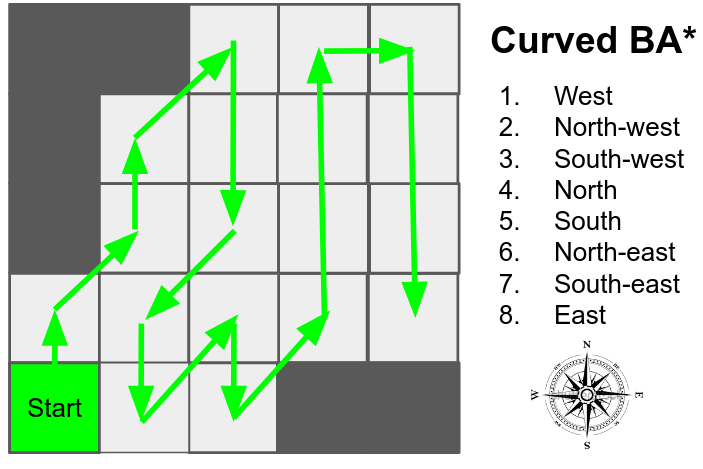
\includegraphics[width=0.6\textwidth]{figures/examplebastarvariant.png}
    \caption{An illustration how the Curved BA* algorithm would solve the CPP. Green arrows are the main path that covers new points.}
    \label{fig:examplebastarvariant}
\end{figure}

\section{Sampling-based BA* and Inward Spiral with Traveling Salesman}
Another approach that were developed to handle covering of a multi floor parking garage is the Sampling-based BA* and Inward Spiral with Traveling Salesman approach. It is based on the idea of the Sampling-Based Coverage Path Planning algorithm described in Section \ref{sec:randomsample}. The general idea is to cover open areas with BA* and more complex areas with Inward Spiral. This is done by covering segments of the area with BA* and Inward Spiral starting from random sampled points and then connect these segments with a Traveling Salesman algorithm. The new algorithm, see \ref{alg:myalgorithm}, follows these steps:

\begin{enumerate}
    \item Use random sampling to get an unvisited $Traversable$ point $p_s$.
    \item For $N_\phi$ different angles $\phi_i$, define $north$ as the angle $\phi_i$ and start covering using the BA* algorithm (Section \ref{sec:BA*impl}) starting from starting point $p_s$. Keep covering until the distance to the next starting point, generated by CPP Step 2, is bigger than a hand tuned threshold, $d_{max}$. See illustration in Figure \ref{fig:myalga}.
    \item Step 2 will generate $N_\phi$ different paths from the same starting point $p_s$. Pick the path that covers the biggest area and add it to a list with paths that covers different segments, $S$.
    \item Repeat the Step 1-3 until a pre defined coverage percentage, $C_1$ or a maximum amount of iterations $N^{iter}_{max}$ has been reached.
    \item Use random sampling to get an unvisited $Traversable$ point $p_s$.
    \item Start covering using the Inward Spiral algorithm (Section \ref{sec:spiral_impl}) starting from starting point $p_s$, see Figure \ref{fig:myalgb}. Keep covering until the distance to the next starting point, generated by CPP Step 2, is bigger than a hand tuned threshold, $d_{max}$. Add the path to $S$.
    \item Repeat the Step 5-6 until a pre defined coverage percentage, $C_2$ has been reached.
    \item Build up a graph tree, $T$, from $S$. Only the start and end positions of the paths in $S$ are added as nodes to $T$. All nodes are connected with edges with weights set to 
    \begin{itemize}
        \item $w=0$, if the edge is between the start and end node of the same path in $S$.
        \item Otherwise, distance based  according to equation 
            \begin{equation}
        \label{eq:distanebased}
            w = w_{offset} + | s_A(x,y) - s_B(x,y) | + K \cdot | s_A(z) - s_B(z) |
        \end{equation}
        where $s_A$ and $s_B$ are the position of the two nodes, $w_{offset}$ is a large number and $K$ is coefficient bigger than 1.
    \end{itemize}
    
     The purpose of $w_{offset}$ is to make sure that the traveling salesman algorithm in the following step always chooses to connect corresponding start and end nodes. Since the environment had multiple floors extra weight is added to difference in height, since the path in most cases will be longer. This is the purpose of coefficent $K$.
    \item Apply a traveling salesman algorithm to calculate the cheapest route, $W_{TSP}$, to visit all nodes in $T$, see Figure \ref{fig:myalgc}. An approximate local search TSP algorithm \cite{python-tsp} was used.
    \item Walk through every node in $W_{TSP}$ and create a ordered list of paths $S_{TSP}$. For every node $s_i$,
    \begin{itemize}
        \item If $s_i$ is a start node, add the corresponding path in $S$ to $S_{TSP}$.
        \item If $s_i$ is a end node, add the corresponding path, but reversed, in $S$ to $S_{TSP}$.
    \end{itemize}
    \item Create a continuous path $W$ by following the paths in $S_{TSP}$. Connect them with obstacle free smooth A* paths, as in CPP Step 3 in previous CPP implementations. See illustration in Figure \ref{fig:myalgd}.
\end{enumerate}

\begin{figure}
\centering
    \begin{subfigure}{\textwidth}
    \centering
    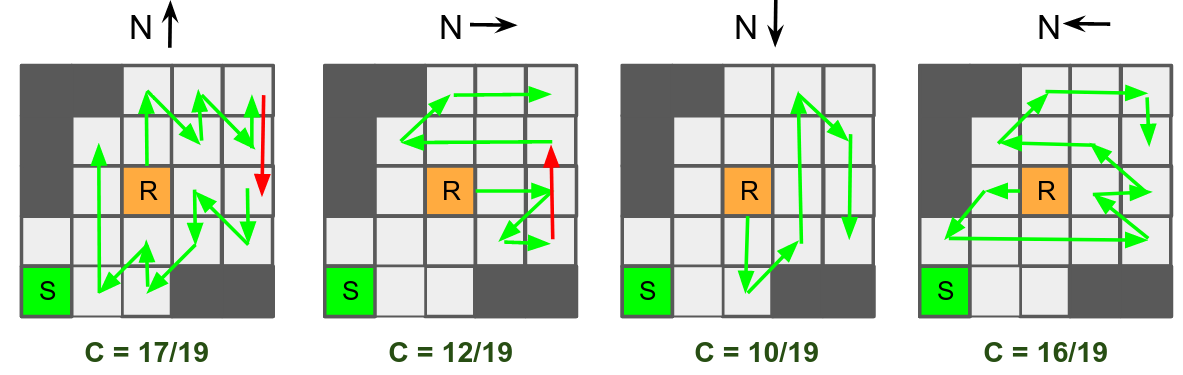
\includegraphics[width=\textwidth]{figures/Sampled_BA.png}
    \caption{For different angles $\phi_i$, define north $N$ as the angle $\phi_i$ and start covering using the BA* starting from random sampled point $R$. Keep covering until the distance to the next starting point is too big. Choose the path with the biggest coverage $C$.}
    \label{fig:myalga}
    \end{subfigure}
    \begin{subfigure}{\textwidth}
    \centering
    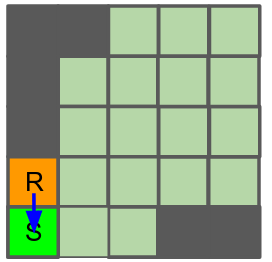
\includegraphics[width=0.3\textwidth]{figures/Sampled_inward.png}
    \caption{Start covering using the Inward Spiral algorithm starting from random sampled uncovered point $R$. Green boxes in the figure are covered by the BA*. See the first path from left in Figure \ref{fig:myalga}.}
    \label{fig:myalgb}
    \end{subfigure}
    \begin{subfigure}{\textwidth}
    \centering
    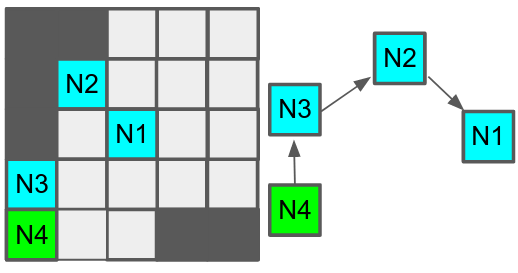
\includegraphics[width=0.55\textwidth]{figures/Sampled_TSP.png}
    \caption{Apply a traveling salesman algorithm to calculate the cheapest route to visit all start and end points of path. Since the weight between start and end node pairs is set to 0 they will always be connected. In this case, the TSP could have chosen the edge $N3\rightarrow N1$ as well since the cost is the same as $N3\rightarrow N2$. The latter was chosen to demonstrate that the path get reversed, see Figure \ref{fig:myalgd}, since $N2$ is an end node.}
    \label{fig:myalgc}
    \end{subfigure}
     \begin{subfigure}{\textwidth}
    \centering
    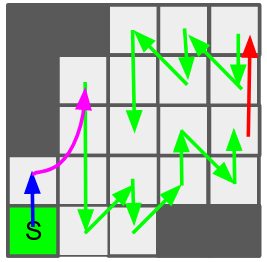
\includegraphics[width=0.3\textwidth]{figures/Sampled_total.png}
    \caption{The final path. The robot follows all paths according to the cheapest route and connects them using smooth A*, see purple arrow. Since $N2\rightarrow N1$ starts from and end node, the path is reversed to the path in \ref{fig:myalga}}
    \label{fig:myalgd}
    \end{subfigure}
    
    \caption{Simplified illustration of the Sampling-based BA* and Inward Spiral with Traveling Salesman algorithm.}
    \label{fig:myalg}
\end{figure}

\begin{algorithm}[H]
\SetAlgoLined
\KwData{Starting position $p_s$, Coverage percentage goals $C_1$ and $C_2$}
\KwResult{Path to cover the area, $W$}
$S = \emptyset$\\
\While{\textup{Coverage $C_1$ or iteration $N^{iter}_{max}$ has not been reached}}{
    $p_r$ = \textup{random uncovered point}\\
    $S_{BA*} = \emptyset$\\
    \For{\textup{angle $\phi \in [0,1, ..., N_{\phi}] \cdot 2\pi/N_{\phi} $ }}{
        \textup{Set $W_{BA*} \rightarrow$ Generated BA* path with north being towards angle $\phi$ starting at $p_r$}\\
        $S_{BA*} = S_{BA*} \cup W_{BA*}$\\
    }
    $W_{best}$ = \textup{Path $W_{BA*}$ in $S_{BA*}$ with the highest coverage} \\
    \If{\textup{Coverage of $W_{best}$ > $C_{min}$}}{
        $S = S \cup W_{best}$  \\
    }
}
\While{\textup{Coverage $C_2$ has not been reached}}{
    $p_r$ = \textup{random uncovered point}\\
    \textup{Set $W_{Spiral} \rightarrow$ Generated Inward Spiral path with starting at $p_r$}\\
    \If{\textup{length of $W_{Spiral}$ > $N_{min}$}}{
        $S = S \cup W_{Spiral}$  \\
    }
}
$T$ = \textup{Empty graph tree}\\
\For{\textup{path $W_i$ in $S$}}{
    \textup{Add start and end point of $W_i$ as nodes in $T$.}
}
$W_{TSP}$ = \textup{Cheapest route to visit all nodes in $T$}\\
\textup{Set $p_{curr} \rightarrow p_s$} \\
$S_{TSP}$ = \emptyset \\
\For{\textup{node $p_i$ in $W_{TSP}$}}{
    \If{\textup{$p_{i}$ is $p_{curr}$}}{
        \textup{\textbf{continue}}
    }
    \eIf{\textup{$p_i$ is a start node}}{
        $W_i$ = \textup{Path in $S$ with $p_i$ as start node} \\
    }{
        $W_i$ = \textup{Reversed path in $S$ with $p_i$ as end node} \\
    }
    $S_{TSP}.\texttt{push\_back}(W_i)$ \\
    \textup{Set $p_{curr} \rightarrow$ Last point in $W_i$} \\
}
$W = \emptyset$ \\
\textup{Set $p_{curr} \rightarrow p_s$} \\
\For{\textup{path $W_i$ in $S_{TSP}$}}{
    $W_{A*}$ = Shortest path from $p_{curr}$ to the start point of $W_i$. \\
    $W = W \cup {W_{A*}, W_i}$ \\
    \textup{Set $p_{curr} \rightarrow$ Last point in $W_i$} \\
}
\textup{\textbf{return $W$}}
 \caption{Sample Based BA* and Inward Spiral with Traveling Salesman.}
 \label{alg:myalgorithm}
\end{algorithm}

\section{Parameters}
\label{sec:param_calc}
All algorithms mentioned in this chapter has multiple parameters that had to be tuned. Most of them needs to be hand tuned or systematically tuned using a large amount of tests. In this section, the values of some of the parameters are motivated using calculations. These values could be used right away, or as a good starting point when tuning.

\subsection{CPP Visited treshold, $r_{visited}$}
CPP Visited treshold $r_{visited}$, is a radius that defines if a position has been visited by the robot and should not be visited again. If this radius is too small, a lot of points will be covered multiple times, which makes the algorithm less efficient. If it is too big, it will be harder for the algorithms to find valid points to go to and consequently miss to cover spots because of inaccessibility.

The radius $r_{visited}$ was set based on the step size and three different scenarios, see Figure \ref{fig:threshold}. It is desired to allow the algorithm to make paths with straight lines side by side. Therefor, $r_{visited}$ should be small enough to allow the scenarios in Figure \ref{fig:threshold_a} and \ref{fig:threshold_c}. However, $r_{visited}$ needs to be big enough to not accept the scenario in Figure \ref{fig:threshold_b}. The distance between two side-by-side paths depends on the third step in the figures. If the distance is big, gaps between the circles allows the algorithm to take steps between the paths, which is unwanted. Therefor, $r_{visited}$ was calculated to make the scenario in Figure \ref{fig:threshold_a}, not allowing any gaps between the side-by-side paths. This value is big enough to not allow the scenario in Figure \ref{fig:threshold_b}, but small enough to allow the scenario in Figure \ref{fig:threshold_c}. Given a step size $\lambda$, $r_{visited}$ is given by
\begin{equation}
    r_{visited} = \frac{\lambda}{\sqrt{2}} \approx 0.71\lambda
    \label{eq:r_visited}
\end{equation}



\begin{figure}
\centering
    \begin{subfigure}{0.3\textwidth}
    \centering
    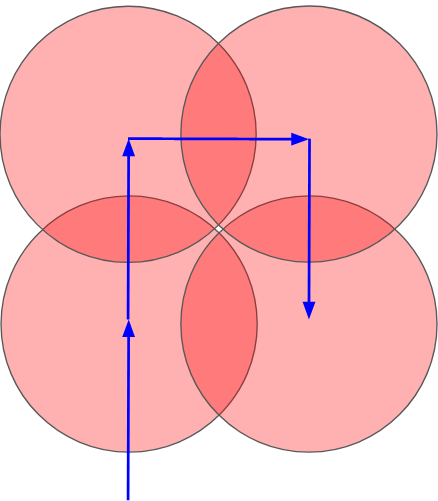
\includegraphics[width=\textwidth]{figures/threshold_a.png}
    \caption{North $\rightarrow$ North $\rightarrow$ East $\rightarrow$ South. Should be accepted and not leave any gaps.}
    \label{fig:threshold_a}
    \end{subfigure}
    \begin{subfigure}{0.3\textwidth}
    \centering
    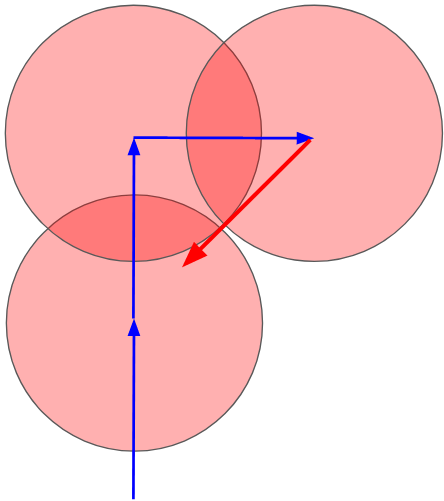
\includegraphics[width=0.96\textwidth]{figures/threshold_b.png}
    \caption{North $\rightarrow$ North $\rightarrow$ East $\nrightarrow$ South-west. Should not be accepted.}
    \label{fig:threshold_b}
    \end{subfigure}
    \begin{subfigure}{0.3\textwidth}
    \centering
    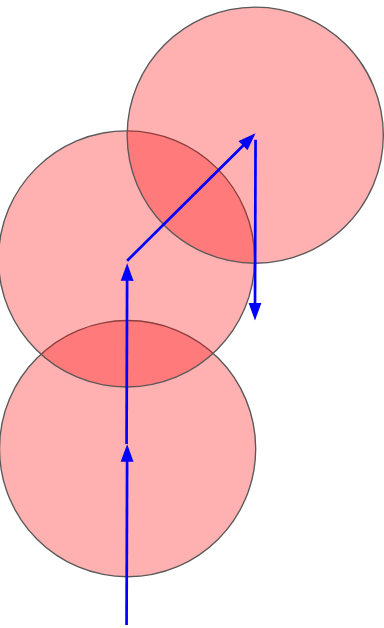
\includegraphics[width=0.8\textwidth]{figures/threshold_c.png}
    \caption{North $\rightarrow$ North $\rightarrow$ North-east $\rightarrow$ South. Should be accepted.}
    \label{fig:threshold_c}
    \end{subfigure}
    \caption{The three different scenarios that was used to define the CPP Visited threshold $r_{visited}$.}
    \label{fig:threshold}
\end{figure}

\subsection{CPP Step size, $\lambda_{CPP}$}
The parameter CPP Step size $\lambda_{CPP}$ defines the length of each step when the algorithms are looking for negihbour. If the world would be represented as a grid instead of point cloud, $\lambda_{CPP}$ would be equivalent to the cell size. Similar to the  $r_{visited}$, a too small $\lambda_{CPP}$ leads to multiple coverage of the same points. A too big $\lambda_{CPP}$ creates gaps between paths, which needs to be visited later and makes the covering path less effective. 

The value of the parameter was set based on the covering radius range of the robot, $r_R$. Two scenarios, see Figure \ref{fig:stepsize}, are possible. If the $\lambda_{CPP}$ in the scenario in Figure \ref{fig:stepsize_a}, would be used in Figure \ref{fig:stepsize_b}, a lot of points would be recovered and make the path inefficient. The opposite would result in a big uncovered gap between the circles in Figure \ref{fig:stepsize_a}. To handle this balance $\lambda_{CPP}$ was simply set to the average between the two scenarios:
\begin{equation}
    \lambda_{CPP} = \frac{\sqrt{2}+2\cos(\pi/8)}{2}r_R \approx 1.63r_R
    \label{eq:lambda_cpp}
\end{equation}


\begin{figure}
\centering
    \begin{subfigure}{0.4\textwidth}
    \centering
    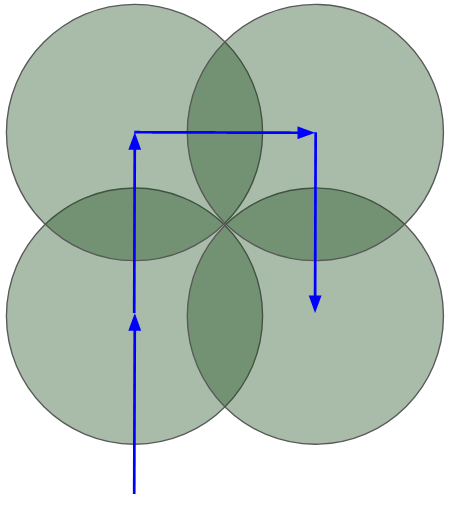
\includegraphics[width=\textwidth]{figures/stepsize_a.png}
    \caption{North $\rightarrow$ North $\rightarrow$ East $\rightarrow$ South. Requires $\lambda_{CPP} = \sqrt{2} \cdot r_R \approx 1.41r_R$ to fill all gaps.}
    \label{fig:stepsize_a}
    \end{subfigure}\hspace{0.1\textwidth}
    \begin{subfigure}{0.4\textwidth}
    \centering
    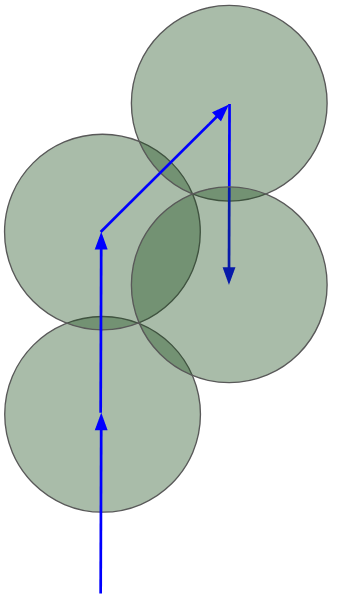
\includegraphics[width=0.67\textwidth]{figures/stepsize_b.png}
    \caption{North $\rightarrow$ North $\rightarrow$ North-east $\nrightarrow$ South. Requires $\lambda_{CPP} = 2\cos(\pi/8) \cdot r_R \approx 1.85r_R$ to fill all gaps.}
    \label{fig:stepsize_b}
    \end{subfigure}
    \caption{The two different scenarios that was used to define the CPP Step size, $\lambda_{CPP}$. Green circles shows the covering range of the robot at each step.}
    \label{fig:stepsize}
\end{figure}